\subsubsection{الگوی \lr{Recursive Containment}}
\label{archRecContainSec}
\begin{RTL}
این الگو \cite{ref4} برای مدیریت سیستم‌های بسیار پیچیده
با نیازمندی‌های فراوان مؤثر است. این الگو شامل شکستن سیستم به
اجزای مرتبط در سطوح مختلف جزئیات است، مانند استفاده از میکروسکوپ
با سطوح مختلف بزرگ‌نمایی. در هر سطح، اشیاء واسط‌هایی
برای همتایان خود فراهم می‌کنند و وظایف را به اجزای کوچک‌تر داخلی
محول می‌کنند، این تجزیه و تحلیل به صورت بازگشتی ادامه می‌یابد
تا هر بخش دارای مسئولیت ساده و متمرکز شود. این رویکرد امکان تجزیه
و تحلیل مقیاس‌پذیر را فراهم می‌کند و سطوح مختلفی از جزئیات رفتار سیستم را ارائه می‌دهد.
\end{RTL}
\begin{figure}[h!]
\centering
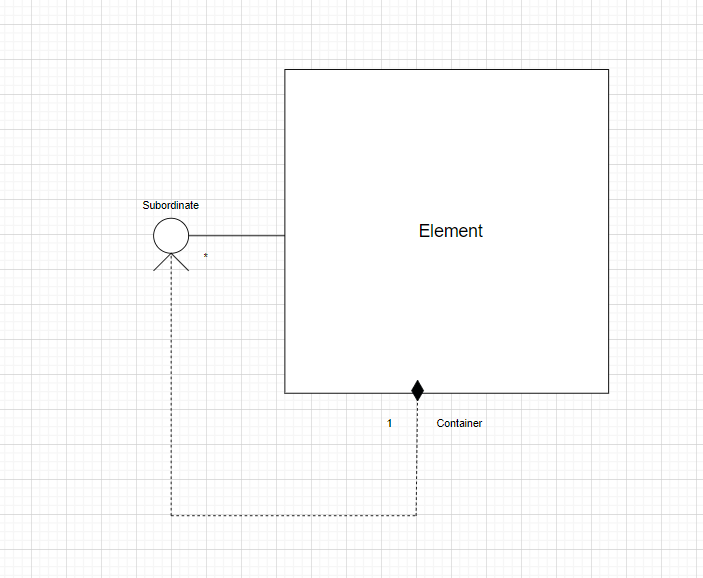
\includegraphics[scale=0.5]{images/first/recursive_contain.png}
\caption{ساختار الگوی \lr{Recursive Containment}}
\end{figure}